\chapter{Introduction}

\section{Problem}
\subsection{Deep Belief Networks can achieve state of the art performance}
% Deep beleif networks are the shit
  % Proven good for images and speech, text analysis (sentimenet analysis)
Deep Belief networks are powerful models that have proven to achieve state of the art performance in many domains. For instance a non-exhaustive list is image classification, dimensionality reduction, natural language recognition, Document classification, Semantic Analysis and .

% Captures deep interactions between complex features. In image domain this is the relationships between pixels.
  % e.g. in an image at best low level layers learn images filters
DBNs capture non-linear interactions between low level features, in the context of image classification the lower layers should capture image filters.

\subsection{DBNs have no mechanism for separating sources}
% Deep belief networks have no way to separate the sources.
Despite a DBNs expressiveness, their is no way to extract these interactions. If an input has multiple sources then the complex combination is instead learnt, the network has no mechanism for extracting multiple causes.
% This is the motivation for this project, we want a way to separate, and model the sources of input data, where said data is a complex combindation of two sources acting independantly.
This is the motivation for this project, to be able to separate the sources of data in a new model.

% Deep Belief Networks are constructed by stacking Restricted Boltzmann Machines (RBMs). This proved a natural starting point for representing two sources. We worked in a shallow environment before attempting to stack RBMs.
\subsection{Restricted Boltzmann Machines cannot separate sources either}
Restricted Boltzmann Machines are two layer, fully connected, unsupervised nueral networks. DBNs are constructed by stacking RBMs. Being the building block of the powerful DBN, RBMs are a natural starting point for representing mutliple sources.
% RBMs make a strong assumption that all features are dependant in the prior, inheriently modelling a single source.
RBMs make the assumption that the features of the input data are dependant in the prior, as they are independant in the posterior. The latter makes them tractable to use in practice, but also means they model/encode a single representation.
  % In the image domain, this equates to all pixels being assumed relevant to what we are trying to model. With enough examples RBMs can generalise, but there is no mechanism for modelling independant subjects.
  Again using the example of images, an input image will map to a single representation, again there is a lack of mechanism for modelling sources that are acting independantly.

% There is another structure, Belief/Bayesian Networks, and the parameterised version, the Sigmoid Belief Network, which makes the polar assumption where each feature is modelled by an independant cause. These are intractable to train in practice.
\subsection{Sigmoid Belief Networks; Intractably rich in practice}
The Sigmoid Belief Network, the parameterized version of a Bayesain/Belief network appears as a natural choice for modelling inpendant sources in that it makes a polar assumption to the RBM; -- Warning Semicolon Use -- Every feature has an independant cause. The sigmoid belief networks assumption could capture data that has multiple sources, but this is intractable in practice.

% Frean, Marsland propose a generative model that aims for a middle ground between these two existing models.
\section{Solution}
\subsection{Trading tractibility for Source Separation}
Frean and Marsland propose a generative model that aims to trade a small amount of the RBMs performance for richness, finding a middle ground between the sigmoid beleif network and the restricted boltzmann machine.
Frean and Marsland also propose an algorithm to invert this model, seperating the sources of an input.

The new generative model, referred to onwards as an ORBM, uses an RBM to model each source and a sigmoid belief network to capture their combination to from data. This project explores the ORBM use for separating two causes.

\begin{figure}[h]
\begin{center}
  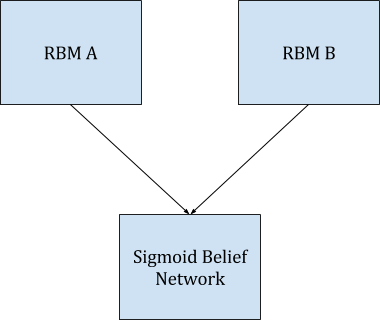
\includegraphics[width = 0.5\textwidth]{Assets/ORBM_fig_1}
\caption{The proposed generative model for capturing two causes, the ORBM.}

\label{F:ORBM-fig-1}
\end{center}
\end{figure}

Given the proposed model and algorithm, this project answers the following questions:
\begin{itemize}
  \item Can this model encode data comprised of more than one cause as it's constituted causes? That is, can the model and new algorithm for inverting it, perform source separation.
  \item Is the ORBMs two cause structure to rich to be tractible in practice?
\end{itemize}
